\chapter{Análise Combinatória} \
		\section{Princípio Fundamental da contagem}
		\begin{list}{\textbf{Questão \arabic{quest}.}}{\usecounter{quest}}
%define a margem da lista.	
%\setlength{\labelwidth}{-2mm} \setlength{\parsep}{0mm}
%\setlength{\topsep}{0mm} \setlength{\leftmargin}{-2mm}
\renewcommand{\labelenumi}{(\alph{enumi})}

		
		\item Thiago possui 3 blusas diferentes e 2 calças diferentes. De quantas maneiras ele poderá escolher uma blusa e uma calça para se vestir?
		
		\item Quantos números de dois algarismos podem ser formados utilizando elementos do conjunto  {1, 2, 3}?
		
		\item Quantos números de dois algarismos diferentes (distintos) podem ser formados utilizando elementos do conjunto {1, 2, 3}?
		
		\item Quantos números de três algarismos podem ser formados utilizando elementos do conjunto {1, 2, 3}?

		\item Quantos números de três algarismos diferentes (distintos) podem ser formados utilizando elementos do conjunto {1, 2, 3}?

		\item Um estádio possui 4 portões. De quantas maneiras diferentes um torcedor pode entrar e sair desse estádio? 
		
		\item Um estádio possui 4 portões. De quantas maneiras diferentes um torcedor pode entrar e sair desse estádio utilizando, para sair, um portão diferente do que entrou? 
		
		\item Mariana desenhou uma bandeira retangular de 3 listras e deseja pintá-la, de modo que duas listras consecutivas não sejam pintadas da mesma cor. Se ela possui 4 lápis de cores diferentes, de quantas maneiras poderá pintar sua bandeira? 
		
		\item Numa prova havia 4 itens para que os alunos respondessem V (verdadeiro) ou F (falso). De quantas maneiras diferentes um aluno que vai “chutar” todas as repostas poderá responder esses itens? 
		
		\item Um painel luminoso retangular é composto por 5 lâmpadas. De quantas maneiras diferentes esse painel pode estar iluminado? (considera-se o painel iluminado se, pelo menos, uma de suas lâmpadas estiver acesa) 
		
		\item Quantos números de 3 algarismo distintos podem ser formados usando-se os algarismo 1,2,3,4 e 5?

		\item Um restaurante oferece no cardápio 2 saladas distintas,e 4 ti podes de pratos de carne,5 variedades de bebidas e 3 sobremesas diferentes. Uma pessoa deseja uma salada,um prato de carne,uma bebida e uma sobremesa.De quantas maneiras a pessoa poderá fazer seu pedido?
		
		\item Quatro times de futebol(Vasco,Atlético,Corinthians e Internacional ) disputam um torneio.Quantos e quais são as possibilidades de classificação para os três primeiros lugares?
		
		\item Numa eleição de uma escola há 3 candidatos a presidente,cinco a vice-presidente,à secretario e 7 a tesoureiro.Quantos podem ser os resultados da eleição?
		
		 \item Com os algarismos 1, 2, 3, 4, 5 e 6, quantos números de três algarismos distintos podemos formar?
		 \begin{multicols}{5}
		 \begin{enumerate}[a)]
		 	\item 30
		 	\item 60
		 	\item 90
		 	\item 120
		 	\item 150
		 \end{enumerate}
		 \end{multicols}

		\item Uma prova consta de 10 questões do tipo V ou F. De quantas maneiras distintas ela pode ser resolvida?
		\begin{multicols}{5}
		 \begin{enumerate}[a)]
		 	\item 128
		 	\item 256
		 	\item 512
		 	\item 1024
		 	\item 2048
		 \end{enumerate}
		 \end{multicols}

		\item Quantos números de três algarismos podemos com os algarismos 0, 1, 2, 3, 4, 5, 6 e 7?
		\begin{multicols}{5}
		 \begin{enumerate}[a)]
		 	\item 348
		 	\item 448
		 	\item 548
		 	\item 648
		 	\item 748
		 \end{enumerate}
		 \end{multicols}

		\item Quantos números ímpares de três algarismos distintos podemos formar com os algarismos 0, 1, 2, 3, 4, 5, 6 e 7?
		\begin{multicols}{5}
		 \begin{enumerate}[a)]
		 	\item 72
		 	\item 144
			\item 200
			\item 240
			\item 288
		 \end{enumerate}
		 \end{multicols}

		\item Um jantar constará de três partes: entrada, prato principal e sobremesa. De quantas maneiras distintas ele poderá ser composto, se há como opções oito entradas, cinco pratos principais e quatro sobremesa?
		\begin{multicols}{5}
		 \begin{enumerate}[a)]
		 	\item 160
		 	\item 150
		 	\item 120
		 	\item 80 
		 	\item 17 
		 \end{enumerate}
		 \end{multicols}
		 
		 \item Se um quarto tem 5 portas, o número de maneiras distintas de se entrar nele e sair dele por um porta diferente é:
		\begin{multicols}{5}
		 \begin{enumerate}[a)]
		 	\item 5
		 	\item 10
		 	\item 15
		 	\item 20
		 	\item 25 
		 \end{enumerate}
		 \end{multicols}

		\item Quantos números de 4 algarismos diferentes têm o algarismo da unidade de milhar igual a 3?
		\begin{multicols}{5}
		 \begin{enumerate}[a)]
		 	\item 1512 
		 	\item 1008
		 	\item 504
		 	\item 3024
		 	\item 2520
		 \end{enumerate}
		 \end{multicols}

		\item Cinco sinaleiros estão alinhados. Cada um tem três bandeiras: uma amarela, uma verde e uma vermelha. Os cinco sinaleiros levantam uma bandeira cada, ao mesmo tempo, transmitindo-se assim um sinal. A quantidade  de sinais diferentes que se pode transmitir é:
		\begin{multicols}{5}
		 \begin{enumerate}[a)]
		 	\item 15
		 	\item 125
		 	\item 243
		 	\item 1215
		 	\item 729 
		 \end{enumerate}
		 \end{multicols}

		\item Com os algarismos 1, 2, 3, 4, 5 e 6 são formados números de quatro algarismos distintos. Dentre eles são divisíveis por 5:
		\begin{multicols}{5}
		 \begin{enumerate}[a)]
		 	\item 20 números
		 	\item 30 números
		 	\item 60 números
		 	\item 120 números
		 	\item 180 números 
		 \end{enumerate}
		 \end{multicols}

		\item Uma estrada de ferro tem 10 estações. Quantos tipos distintos de bilhetes existem em circulação, sabendo-se que cada bilhete contém impressos apenas a estação de partida e a estação de chegada? (Supondo que o trem tem vagões de apenas uma classe)
		\begin{multicols}{5}
		 \begin{enumerate}[a)]
		 	\item 28
		 	\item 45 
		 	\item 20
		 	\item 56
		 	\item 90
		 \end{enumerate}
		 \end{multicols}

		
			\item Num banco de automóvel, o assento pode ocupar seis posições diferentes enquanto o encosto pode ser colocado em cinco posições. Combinando assento e encosto, quantas posições diferentes esse banco pode ter?
				\begin{enumerate}
					\begin{multicols}{5}
					\item 6	
	  				\item 30	
	  				\item 90
	  				\item 180 
	  				\item 720		
	  				\end{multicols}
				\end{enumerate}			

			\item Um trem de passageiros é constituído de um a locomotiva e seis vagões distintos, sendo um deles restaurante. Sabendo-se que a locomotiva deve ir à frente e que o vagão restaurante não pode ser colocado imediatamente após a locomotiva, o número de modos diferentes de montar a composição é:
			\begin{enumerate}
					\begin{multicols}{5}
					\item 120
	  				\item 230
	  				\item 500
	  				\item 600
	  				\item 720		
	  				\end{multicols}
				\end{enumerate}

		\item Para participar de um campeonato de futebol, o técnico da Fatec selecionou 22 jogadores, 2 para cada posição. O número de maneiras distintas que o técnico pode formar esse time de modo que nenhum jogador atue fora de sua posição é:
		\begin{enumerate}
					\begin{multicols}{5}
					\item 2541
	  				\item 2048
	  				\item 462
	  				\item 231
	  				\item  44		
	  				\end{multicols}
				\end{enumerate}

		\item Maria pretende distribuir 11 maças entre duas pessoas de modo que cada pessoa receba ao menos uma maça. De quantas maneiras distintas isso pode ser feito?

		\item O mapa abaixo representa a divisão do Brasil em suas regiões. O mapa deve ser colorido de maneira que regiões com uma fronteira em comum sejam coloridas com cores distintas. Determine o número (n) de maneiras de se colorir o mapa, usando-se 5 cores.
		\begin{center}
		 	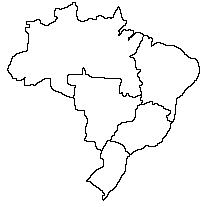
\includegraphics[scale=0.8]{figuras/fig16.png}
		\end{center}
		
		\item (Unesp-00) Um turista, em viagem de férias pela Europa, observou pelo mapa que, para ir da cidade A à cidade B, havia três rodovias e duas ferrovias e que, para ir de B até uma outra cidade, C, havia duas rodovias e duas ferrovias. O número de percursos diferentes que o turista pode fazer para ir de A até C, passando pela cidade B e utilizando rodovia e trem obrigatoriamente, mas em qualquer ordem, é:
		\begin{enumerate}
					\begin{multicols}{5}
					\item 9
	  				\item 10
	  				\item 12
	  				\item 15
	  				\item 20		
	  				\end{multicols}
				\end{enumerate}

		\item Em uma lanchonete, os sorvetes são divididos em três grupos: o vermelho, com 5 sabores; o amarelo, com 3 sabores; e o verde, com 2 sabores. Pode-se pedir uma casquinha com 1, 2 ou 3 bolas, mas cada casquinha não pode conter 2 bolas de um mesmo grupo. O número de maneiras distintas de se pedir uma casquinha é:
		\begin{enumerate}
					\begin{multicols}{4}
					\item 86
	  				\item 131
	  				\item 61
	  				\item 71 		
	  				\end{multicols}
				\end{enumerate}

		\item Uma prova de vestibular tem 100 testes com cinco alternativas cada um. De quantos modos o cartão de respostas poderá ser preenchido, marcando aleatoriamente apenas uma alternativa em cada questão?

		\item Duas das 50 cadeiras de uma sala serão ocupadas por dois alunos. Qual é o número de maneiras distintas possíveis que esses alunos terão para escolher duas das 50 cadeiras?

		\item Um código usado para identificar componentes consiste em oito símbolos para cada componente. Os dois primeiros símbolos são duas letras de um alfabeto de 24 letras e as seis posições restantes são ocupadas por algarismos da nossa numeração. Quantos objetos distintos podem ser codificados?
		\begin{enumerate}
					\begin{multicols}{5}
					\item 576 milhões
	  				\item 306.110.000
	  				\item 48 milhões
	  				\item 57.600
	  				\item 28.800		
	  				\end{multicols}
				\end{enumerate}

		\item Suponha que 32 seleções disputem um campeonato mundial, sem divisão de chaves. Quantas são as possibilidades matemáticas de classificação dos três primeiros lugares?

		\item (Unicamp) Sabendo que os números de telefone não começam com zero e nem com 1, quantos números diferentes de telefone podem ser formados com sete algarismos?

		\item (Unesp-03) Na convenção de um partido para lançamento da candidatura de uma chapa ao governo de certo estado havia 3 possíveis candidatos a governador, sendo dois homens e uma mulher, e 6 possíveis candidatos a vice-governador, sendo quatro homens e duas mulheres. Ficou estabelecido que a chapa governador/vice-governador seria formada por duas pessoas de sexos opostos. Sabendo que os nove candidatos são distintos, o número de maneiras possíveis de se formar a chapa é
		\begin{enumerate}
					\begin{multicols}{5}
					\item 18
	  				\item 12
	  				\item 8
	  				\item 6
	  				\item 4		
	  				\end{multicols}
				\end{enumerate}

		\item Quantos números de 4 algarismos do sistema decimal 
			\begin{enumerate}
				\item são ímpares?
				\item são pares e todos os algarismos são distintos?
			\end{enumerate}

		\item (Mack) Com os algarismos 1, 2, 3, 4 e 5 e sem repetição, podemos escrever x números maiores do que 2500. Calcule x.

		\item Quantos números de 4 algarismos do sistema decimal
			\begin{enumerate}
				\item tem pelo menos dois deles repetidos?	
				\item tem pelo menos três deles repetidos?	
			\end{enumerate}
		\end{list}
		
		\section{Princípio Multiplicativo}
		\begin{list}{\textbf{Questão \arabic{quest}.}}{\usecounter{quest}}
%define a margem da lista.	
%\setlength{\labelwidth}{-2mm} \setlength{\parsep}{0mm}
%\setlength{\topsep}{0mm} \setlength{\leftmargin}{-2mm}
\renewcommand{\labelenumi}{(\alph{enumi})}

		\item Quantos números de 3 algarismos distintos, múltiplos de 5 podemos escrever com \{1, 3, 5, 7, 9\}.

		\item (Unifor) Um casal e seus quatro filhos vão ser colocados lado a lado para tirar uma foto. Se todos os filhos devem ficar entre os pais, de quantos modos distintos os seis podem posar para a foto?

		\item A figura a seguir representa uma bandeira com 4 listras. Dispondo-se de 4 cores distintas, deseja-se pintar todas as listras, de forma que listras vizinhas tenham cores diferentes.
		\begin{center}
		
\includegraphics[scale=0.5]{figuras/fig23.png}
		\end{center}
		De quantas maneiras distintas a bandeira pode ser pintada? Justifique.		

		\item (Fuvest) Quantos números de 5 algarismos podemos escrever com \{2, 4, 6, 8\} de modo que dois algarismos adjacentes quaisquer sejam diferentes?		

		\item (Mack) O total de números formados com algarismos distintos maiores do que 50000 e menores do que 90000 e que são divisíveis por 5 é:
		\begin{multicols}{5}		
		\begin{enumerate}
			\item 1596
			\item 2352
			\item 2686
			\item 2688
			\item 4032
		\end{enumerate}
		\end{multicols}

		\item (FGV) Usando os algarismos 1, 3, 5, 7 e 9, existem x números de quatro algarismos de modo que pelo menos dois algarismos sejam iguais. Qual é o valor de x?

		\item Determine quantos números naturais pares, de 3 algarismos podemos formar utilizando os dígitos:
		\begin{multicols}{2}
		\begin{enumerate}
		\item 1, 2, 3, 4, 5, 6 e 7.
		\item 0, 1, 2, 3, 4, 5, 6 e 7.
		\end{enumerate}
		\end{multicols}

		\item Utilizando os algarismos 1, 2, 3, 4, 5, 6 e 7 sem repetição quantos números naturais compreendidos entre 300 e 3000 podemos formar?

		\item (Unicamp-02) Em Matemática, um número natural a é chamado palíndromo se seus algarismos, escritos em ordem inversa, produzem o mesmo número. Por exemplo, 8, 22 e 373 são palíndromos. Quantos números naturais palíndromos existem entre 1 e 9.999?

		\item (Puccamp) Com os elementos do conjunto A = \{1, 2, 3, 4, 5, 6\} são formados números de 3 algarismos distintos. A quantidade de números obtidos cuja soma dos algarismos é par é:
		\begin{multicols}{5}
		\begin{enumerate}
			\item 30
			\item 36
			\item 52
			\item 60
			\item 72
		\end{enumerate}
		\end{multicols}
	
		\end{list}	
		\section{Atividades Básicas}				
			\begin{list}{\textbf{Questão \arabic{quest}.}}{\usecounter{quest}}
%define a margem da lista.	
%\setlength{\labelwidth}{-2mm} \setlength{\parsep}{0mm}
%\setlength{\topsep}{0mm} \setlength{\leftmargin}{-2mm}
\renewcommand{\labelenumi}{(\alph{enumi})}
	
		
	\item Um homem vai a um restaurante disposto a comer um só prato de carne e uma só sobremesa. O cardápio oferece oito pratos distintos de carne e cinco pratos diferentes de sobremesa. De quantas formas pode o homem fazer sua refeição?
	
	\item Uma moça possou 5 blusas e 6 saias. De quantas formas ele pode vestir uma blusa e uma saia?
	
	\item Num festa existem 80 homens e 90 mulheres. Quantos casais diferentes podem ser formados?
	
	\item Um edifício tem 8 portas. De quantas formas uma pessoa poderá entrar no edifício e sair por uma porta diferente da que usou para entrar?
	
	\item Um homem possui 10 ternos, 12 camisas e 5 pares de sapatos. De quantas formas poderá ele vestir um terno, uma camisa e um par de sapatos?
	
	\item De quantas formas podemos responder a 12 perguntas de um questionário, cujas respostas para cada pergunta são: sim o não?
	
	\item Uma prova consta de 20 testes tipo Verdadeiro ou Falso. De quantas formas uma pessoa poderá responder os 20 testes?
	
	\item Quantos anagramas podemos formar, batendo ao acaso em 6 teclas (escolhidas entre as 26 existentes) num teclado? Entre eles consta o anagrama TECTEC?
	
	\item Num concurso para preenchimento de uma cátedra, apresentam-se 3 candidatos. A comissão julgador é constituída de 5 membros, devendo cada examinador escolher exatamente um candidato. De quantos modos os votos desses examinadores podem ser dados?
	
	\item Quantos números de 3 algarismos (iguais ou distintos) podemos formar com os dígitos 1, 2, 3, 7 e 8?
	
	\item Temos um conjunto de 10 nomes e outro de 20 sobrenomes. Quantas pessoas podem receber um nome e um sobrenome, com esses elementos?
	
	\item Cinco moedas são lançadas. Quantas sequencias possíveis de caras e coroas existem?
	
	\item Seis dados são lançados simultaneamente. Quantas sequencias de resultados são possíveis, se considerarmos cada elemento de sequencia como o número obtido em cada dado?
	
	\item Quantos números telefônicos com 7 dígitos podem ser formados, se usarmos os dígitos de 0 a 9?
	
	\item As letras do código MORSE são formadas por sequencias de traços ($-$) e pontos ($\cdot$) sendo permitidas repetições. Por exemplo: ($-$,$\cdot$,$-$,$-$,$\cdot$,$\cdot$).
	
	Quantas letras podem ser representadas:
	\begin{enumerate}[a)]
		\item usando exatamente 3 símbolos:
		\item usando no máximo 8 símbolos?
	\end{enumerate}	 
	
	\item Nayara vai à praia e com um maiô e uma canga. Sabendo que ela possui sete cangas diferentes e quatro maiôs, determine o número de maneiras distintas que a Nayara tem para se vestir para ir à praia.
	
	\item Dispondo dos algarismos 2,4,6 e 8, quantos números naturais de 4 algarismos podemos formar?
	
	\item Em uma classe possui 18 meninos e 20 meninas. Quantos casais diferentes podem ser formados para a festa junina do colégio?
	
	\item Uma mansão possui 9 portas que dão acesso ao seu interior. De quantas maneiras uma pessoa pode entrar na mansão e sair por uma porta diferente da que usou para entrar?
	
	\item Quantos números distintos de três algarismos podemos formar com os números: 1,3,5,7 e 9 ?
	
	\item Ana e Lucas vão se casar e precisam entregar os convites de casamento para os padrinhos. Sabe-se que 6 padrinhos moram em uma cidade X, cada um em um bairro: A, B, C, D, E, F. Encontre o número de maneiras distintas que os noivos tem para entregar os convites para esses padrinhos, sabendo que vai começar pelo bairro C e terminar com o bairro F?
	
	\item Uma bandeira é formada por seis listras, que devem ser pintadas por quatro cores diferentes. De quantas maneiras será possível pintá-la sendo que, duas listras adjacentes não sejam da mesma cor?
	
	\item Temos dois conjuntos: A e B. Sabe-se que o conjunto A é formado por 12 nomes de garotas e no conjunto B por 30 adjetivos. Então, quantas possibilidades diferentes podemos ter de uma garota e seu adjetivo relacionados?
	
	\item De quantas maneiras uma garota pode responder 10 perguntas, cujas respostas só pode ser sim ou não?
	
	\item Agilson é um homem de negócios e possui 10 ternos, 20 camisas, 30 gravatas e 5 pares de sapatos. De quantas maneiras ele poderá se arrumar para uma reunião importante, sendo que vai usar um terno, uma camisa, uma gravata e um par de sapato?	
	
	
	\item As placas dos automóveis são formadas por três letras seguidas de quatro algarismos. Na cidade Michelês, as placas só podem ser formadas por algarismos pares (0,2,4,6,8) e as letras do nome da própria cidade , sem repetição em ambos. Quantas placas distintas possui nessa cidade?
	
	\item Em uma cidade do interior de São Paulo, os números dos telefones têm 8 algarismos. Os quatro primeiros constituem o prefixo. Sabendo que em todas as padarias os quatro últimos dígitos são o número três e o prefixo não tem dígitos repetidos, determine o número de telefones que podem ser instalados nas padarias dessa cidade.
	
	\item Em um cinema há 7 cadeiras livres e consecutivas. De quantas maneiras sete pessoas podem escolher os seus assentos, sendo que João Pedro e Gianluca não podem se sentar um do lado do outro?
	
\end{list}	

\section{Atividades Básicas: Parte II}				
	\begin{list}{\textbf{Questão \arabic{quest}.}}{\usecounter{quest}}
%define a margem da lista.	
%\setlength{\labelwidth}{-2mm} \setlength{\parsep}{0mm}
%\setlength{\topsep}{0mm} \setlength{\leftmargin}{-2mm}
\renewcommand{\labelenumi}{(\alph{enumi})}
	
	
	\item (Unesp-00) Um turista, em viagem de férias pela Europa, observou pelo mapa que, para ir da cidade A à cidade B, havia três rodovias e duas ferrovias e que, para ir de B até uma outra cidade, C, havia duas rodovias e duas ferrovias. O número de percursos diferentes que o turista pode fazer para ir de A até C, passando pela cidade B e utilizando rodovia e trem obrigatoriamente, mas em qualquer ordem, é:
	\begin{enumerate}
		\begin{multicols}{5}
			\item 9
	  		\item 10
	  		\item 12
	  		\item 15
	  		\item 20
	  \end{multicols}
	\end{enumerate}
 
	\item Um código usado para identificar componentes consiste em oito símbolos para cada componente. Os dois primeiros símbolos são duas letras de um alfabeto de 24 letras e as seis posições restantes são ocupadas por algarismos da nossa numeração. Quantos objetos distintos podem ser codificados?
	\begin{enumerate}
		\begin{multicols}{5}
			\item 576 milhões
	  		\item 306.110.000
	  		\item 48 milhões
	  		\item 57.600
	  		\item 28.800
	  \end{multicols}
	\end{enumerate}
	
	\item Suponha que 32 seleções disputem um campeonato mundial, sem divisão de chaves. Quantas são as possibilidades matemáticas de classificação dos três primeiros lugares?

	\item (Unicamp) Sabendo que os números de telefone não começam com zero e nem com 1, quantos números diferentes de telefone podem ser formados com sete algarismos?

	\item (Unesp-03) Na convenção de um partido para lançamento da candidatura de uma chapa ao governo de certo estado havia 3 possíveis candidatos a governador, sendo dois homens e uma mulher, e 6 possíveis candidatos a vice-governador, sendo quatro homens e duas mulheres. Ficou estabelecido que a chapa governador/vice-governador seria formada por duas pessoas de sexos opostos. Sabendo que os nove candidatos são distintos, o número de maneiras possíveis de se formar a chapa é
	\begin{enumerate}
		\begin{multicols}{5}
			\item 18
	  		\item 12
	  		\item 8
	  		\item 6
	  		\item 4
	  \end{multicols}
	\end{enumerate}
	
	\item Quantos números de 4 algarismos do sistema decimal:
	\begin{enumerate}		
			\item são ímpares?
	  		\item são pares e todos os algarismos são distintos?	  			
	\end{enumerate}
	
	\item (Mack) Com os algarismos 1, 2, 3, 4 e 5 e sem repetição, podemos escrever x números maiores do que 2500. Calcule x.

	\item Quantos números de 4 algarismos do sistema decimal:
	\begin{enumerate}
		\begin{multicols}{2}
			\item tem pelo menos dois deles repetidos?
	  		\item tem pelo menos três deles repetidos?	  		
	  \end{multicols}
	\end{enumerate}
	
	\end{list}	
\section{Combinações}
\begin{list}{\textbf{Questão \arabic{quest}.}}{\usecounter{quest}}
%define a margem da lista.	
%\setlength{\labelwidth}{-2mm} \setlength{\parsep}{0mm}
%\setlength{\topsep}{0mm} \setlength{\leftmargin}{-2mm}
\renewcommand{\labelenumi}{(\alph{enumi})}

\item Uma escola tem 9 professores de matemática. Quatro deles deverão representar a escola em um congresso. Quantos grupos de 4 são possíveis? 

\item Resolver a equação $C_{x, 2} = 3$.

\item Dos 12 jogadores levados para uma partida de vôlei, apenas 6 entrarão em quadra no início do jogo. Sabendo que 2 são levantadores e 10 são atacantes, como escolher 1 levantador e 5 atacantes?

\item De quantos modos podemos escolher 2 objetos em um grupo de 6 objetos distintos?

\item De quantas maneiras podemos escolher 2 estudantes numa classe com 30 alunos?

\item De quantas maneiras podemos dividir 10 rapazes em dois grupos de cinco?

\item Em uma sala de aula existem 12 alunas, onde uma delas chama-se Carla, e 8 alunos, onde um deles atende pelo nome de Luiz. Deseja-se formar comissões de 5 alunas e 4 alunos. Determine o número de comissões, onde simultaneamente participam Carla e Luiz.

\item Um pesquisador científico precisa escolher três cobaias, num grupo de oito cobaias. Determine o número de maneiras que ele pode realizar a escolha.

\item No jogo de basquetebol, cada time entra em quadra com cinco jogadores. Considerando-se que um time para disputar um campeonato necessita de pelo menos 12 jogadores, e que desses, 2 são titulares absolutos, determine o número de equipes que o técnico poderá formar com o restante dos jogadores, sendo que eles atuam em qualquer posição.

\item Uma sala de aula possui 6 lâmpadas. De quantas maneiras diferentes essa sala pode ficar iluminada?
Um time de futebol é composto de 11 jogadores, sendo 1 goleiro, 4 zagueiros, 4 meio campistas e 2 atacantes. Considerando-se que o técnico dispõe de 3 goleiros, 8 zagueiros, 10 meio campistas e 6 atacantes, determine o número de maneiras possíveis que esse time pode ser formado.

\end{list}
	